\documentclass{article}

% ---------------------------------------------------------------------------------------------------------------
% Atlas-5K growth paper (1M -> 10M -> 24M), NeurIPS format with appendix and paper checklist.
% Build: python figs4.py && python make_tables.py --check && pdflatex main && bibtex main && pdflatex main && pdflatex main
% Every number is copied from a run log or result file in data/ or ../results/colab/atlas5k_grown/; the appendix tables
% are generated from those files (make_tables.py), and --check verifies Tables 1-3 below against them.
% Rules and predictions are in atlas/README.md, committed to GitHub before the runs they govern (Appendix H).
% ---------------------------------------------------------------------------------------------------------------
\newif\ifpreprint
\preprinttrue
\ifpreprint
  \usepackage[preprint]{neurips_2025}
\else
  \usepackage{neurips_2025}
\fi
\makeatletter\renewcommand{\@noticestring}{Preprint.}\makeatother % not under review anywhere: replace the style's "Preprint. Under review."

\makeatletter
\renewcommand{\@neuripsordinal}{41st}
\renewcommand{\@neuripsyear}{2027}
\makeatother

\usepackage[utf8]{inputenc}
\usepackage[T1]{fontenc}
\usepackage{hyperref}
\usepackage{url}
\usepackage{booktabs}
\usepackage{float}
\usepackage{amsfonts,amsmath,amssymb,amsthm}
\usepackage{microtype}
\usepackage{xcolor}
\usepackage{graphicx}
\usepackage{caption}
\captionsetup{font=small,labelfont=bf}
\usepackage{enumitem}
\setlist{leftmargin=1.3em,itemsep=1pt,topsep=2pt}
\definecolor{atlasblue}{HTML}{1F5FBF}
\hypersetup{colorlinks=true,linkcolor=atlasblue!75!black,citecolor=atlasblue!75!black,urlcolor=atlasblue!75!black}
\newtheorem{proposition}{Proposition}

\title{Grow, Don't Restart: Compact Station World Models, Grown from 1M to 24M Parameters, Beat TimesFM and Chronos on WEATHER-5K}

\ifpreprint
\author{%
  Aditya Kumar \qquad Anupam Singh\\
  ParadoxAI Lab\\
  \texttt{contact.paradoxailab@gmail.com}
}
\else
\author{Anonymous Author(s)\\Affiliation\\Address\\\texttt{email}}
\fi

\begin{document}
\maketitle

\begin{abstract}
Time-series foundation models with up to 205M parameters are increasingly used zero-shot for weather-station
forecasting. We test whether a compact, task-trained world model that is \emph{grown} rather than restarted can beat
them under paired statistical tests. Atlas-5K is a station-graph model: each station reads its last 48 hours together
with its 31 nearest neighbours, the model encodes them into a latent state, and one shared transition with
geometry-biased attention rolls the state forward. We grow an adopted 0.97M-parameter Atlas twice with exact,
function-preserving maps: to 9.64M (width tiled with zero-sum perturbations, new blocks as the identity), then to
24.1M (each block's hidden layer widened 2.5$\times$ with zero-output units, one block added). Every rule and numeric
prediction was committed to a public repository before the run it governs. On WEATHER-5K at 24 hours we compare both
grown models, on identical windows at 709 stations, with nine foundation-model configurations (TimesFM~2.5 and 3.0,
Chronos-2 univariate and multivariate, Chronos-Bolt, TiRex, Sundial, Time-MoE and TTM) and persistence. Both models win
all 50 model--variable comparisons (station-block bootstrap and Diebold--Mariano, Holm-corrected, $\alpha=0.01$) on the
2023 test year and on 19 months of NOAA observations from 2024--25 that Atlas never saw. The 24.1M model's standardised
error is 17.0\% below the best foundation model, TimesFM~3.0, and its per-variable error is 9--48\% below every
foundation model. On the full 2023 test it has lower error than the benchmark's best published model, PhysicsFormer
(19.3M), on four of five variables, but higher error on sea-level pressure, where ECMWF's operational forecast remains
far ahead. Size bought little: 10$\times$ the parameters gave $-1.95\%$ validation error and a further 2.5$\times$ gave
$-1.03\%$, with no significant gain on pressure. We report every prediction, including the two that failed, and
release the code, rules, logs and weights.
\end{abstract}

\section{Introduction}

Station forecasting means predicting the next hours of temperature, humidity, wind and pressure where they are
measured. Two families of models compete for this job. Global numerical and AI weather models
\citep{lam2023graphcast,bi2023pangu,lang2024aifs} forecast gridded fields that are then interpolated to stations.
Time-series foundation models (TSFMs) such as TimesFM \citep{das2024timesfm,timesfm25,timesfm3} and Chronos
\citep{ansari2024chronos,ansari2025chronos2,chronosbolt} forecast any series zero-shot from its own history.
WEATHER-5K \citep{han2026weather5k} provides a common test bed: 5,672 stations from NOAA's Integrated Surface Database
\citep{smith2011isd}, hourly from 2014 to 2023, a fixed split, and published scores up to the ECMWF-HRES forecast at the
stations.

We ask three questions. \textbf{(i)} Can a compact model trained for this task beat 35--205M-parameter TSFMs under
paired tests on identical windows, rather than by comparing reported numbers? \textbf{(ii)} When more capacity is
wanted, can one grow the trained model instead of restarting, without losing what it has learned? \textbf{(iii)} How
much does size still buy at 10--25M parameters on 16.6M training station-days?

\paragraph{Contributions.}
\begin{itemize}
\item Two exact growth maps for a station-graph transformer (Section~\ref{sec:grow}, proof in Appendix~\ref{app:proofs}):
width tiling with zero-sum perturbations, and hidden-layer widening with zero-output units plus identity blocks. The
grown models reproduce their parents' forecasts to within $3\times10^{-5}$ at the start of training.
\item A pre-registered, paired head-to-head of two grown models against nine TSFM configurations from six groups and
persistence, over the 2023 test year and a 19-month period after the benchmark ends (Section~\ref{sec:h2h}). Both
models win all 50 comparisons in each period.
\item An account of what size bought, with every pre-registered prediction scored (Section~\ref{sec:pred},
Appendix~\ref{app:prereg}), and the code, logs, per-window errors and weights released.
\end{itemize}
The 24.1M model is released as ``Atlas-5K 25M''; we call it the 24M model here.

\section{Related work}

\textbf{Station and time-series forecasting.} DLinear \citep{zeng2023dlinear}, PatchTST \citep{nie2023patchtst} and
iTransformer \citep{liu2024itransformer} model each series without the stations' geometry. WEATHER-5K also reports
physics-informed variants, of which PhysicsFormer is the strongest \citep{han2026weather5k}. Spatio-temporal graph
models \citep{li2018dcrnn,wu2019graphwavenet,shao2022stid} share information between sensors through a graph, as Atlas
does through attention biased by geometry.

\textbf{Time-series foundation models.} TimesFM \citep{das2024timesfm}, Chronos \citep{ansari2024chronos}, Chronos-2
\citep{ansari2025chronos2}, Moirai \citep{woo2024moirai}, Lag-Llama \citep{rasul2023lagllama}, MOMENT
\citep{goswami2024moment}, Toto \citep{cohen2024toto}, Sundial \citep{liu2025sundial}, Time-MoE \citep{shi2025timemoe},
TTM \citep{ekambaram2024ttm} and TiRex \citep{auer2025tirex} are pretrained on large corpora and used zero-shot.
GIFT-Eval \citep{aksu2024gifteval} ranks them across domains. We compare on one domain, against ten configurations of
these models run under their documented settings.

\textbf{Growing networks and scaling.} Function-preserving growth began with Net2Net \citep{chen2016net2net} and was
extended to transformers \citep{gong2019stacking,chen2022bert2bert,wang2023ligo}. Our first map differs from Net2Net's
duplication by a zero-sum perturbation that breaks the symmetry between copies without changing the function; our
second needs no symmetry breaking. Scaling laws \citep{kaplan2020scaling,hoffmann2022chinchilla} describe when size
pays; we add two measured points for a small spatial model.

\section{Atlas-5K}
\label{sec:model}

\textbf{Inputs.} For station $s$ and forecast start $t$, the model reads a 32-station neighbourhood: $s$ and its 31
nearest stations on the sphere (median radius 352\,km). For each station it takes 48 hours of the five variables,
standardised by the benchmark's scaler, a mask of observed values (missing values are not filled), and sine and cosine
features of the hour of day and day of year for the 48 input and 24 output hours. Static inputs are latitude,
longitude and elevation; pair inputs are the east and north offsets and the distance between every two stations.

\textbf{Model.} A linear map embeds each station's window into a $d$-dimensional state. Pre-LayerNorm residual blocks
$x\mapsto x+B\,\mathrm{GELU}(A\,\mathrm{LN}(x))$ with hidden width $rd$ encode it, interleaved with attention among the
32 stations whose logits carry a per-head bias computed by a small network from the pair geometry. The latent dynamics
apply \emph{one} shared transition six times, each step covering four forecast hours: the step's time features are
added, $n_d$ residual blocks and the spatial attention update the state, and a linear decoder reads that step's hours.
The median forecast is the last observed value plus the decoded correction; the 10\% and 90\% quantiles are the median
minus and plus learned non-negative spreads, so they cannot cross. Training minimises the pinball loss
\citep{koenker1978quantile} plus 0.2 times the error of reconstructing 15\% of the observed inputs, hidden at random.
The median is the forecast that is scored.

\textbf{The 1M parent (v2c).} $d=196$, 4 heads, $r=2$, two encoder and two dynamics blocks: 968,672 parameters,
trained from scratch on all 2014--2021 days (2,920 days $\times$ 5,672 stations $=16.6$M station-days).

\section{Growing Atlas twice}
\label{sec:grow}

\textbf{1M$\to$10M: width.} Every stream vector is tiled, $z'=[z;z]$. For LayerNorm \citep{ba2016layernorm} with gain
and bias tiled, $\mathrm{LN}([z;z])=[\mathrm{LN}(z);\mathrm{LN}(z)]$, because $[z;z]$ has the mean and variance of $z$.
Layers that write the stream have their output rows tiled. Layers that read it get input columns
$[W/2+\varepsilon,\;W/2-\varepsilon]$, so $[W/2+\varepsilon,\,W/2-\varepsilon][u;u]=Wu$ exactly while the two copies
can receive different gradients; with Net2Net's plain duplication they would stay identical. Attention heads are tiled
per head, so head size and scale are unchanged. New encoder and dynamics blocks are appended with $B=0$, so each starts
as the identity. Result: $d=392$, 8 heads, 7+7 blocks, \textbf{9,639,780} parameters.

\textbf{10M$\to$24M: hidden width and depth.} Tiling the stream again would give about 38M parameters, and a
non-integer factor would change LayerNorm's statistics. Instead, each block's hidden layer is widened from $2d$ to $5d$
units (784$\to$1,960): $A'=[A;A_{\text{new}}]$, $B'=[B,\,0]$, with $A_{\text{new}}$ drawn from the larger model's
initialisation. One encoder block is appended as the identity. Result: 8+7 blocks, \textbf{24,103,796} parameters.

\begin{proposition}\label{prop:grow}
With the perturbations summing to zero over copies (Map~1) or $B_{\text{new}}=0$ (Map~2), the grown network computes the
same function as its parent in exact arithmetic. Under Map~2, at the first step $\partial L/\partial B_{\text{new}}$ is
generically non-zero while $\partial L/\partial A_{\text{new}}=0$; $A_{\text{new}}$ receives gradient from the second
step on.
\end{proposition}
Appendix~\ref{app:proofs} gives the proof. In floating point, the largest output difference on random inputs was
$2.6\times10^{-5}$ (Map~1, outputs of about 1.2) and $1.8\times10^{-5}$ (Map~2, outputs of about 2.5): summation order only.

\textbf{Continued training.} AdamW \citep{loshchilov2019adamw}, 3\% warm-up then one-cycle decay
\citep{smith2019onecycle}, 80,000 steps of 256 neighbourhoods, weight decay $10^{-4}$, gradient clipping at 1.0,
mixed precision, validation every 2,000 steps on 300 fixed stations, best checkpoint kept, seed 600. Peak learning rate
$3\times10^{-4}$ for the 10M and $2\times10^{-4}$ for the 24M, written down before each run. Hardware and times are in
Appendix~\ref{app:train}.

\section{Protocol}
\label{sec:protocol}

\textbf{Benchmark.} WEATHER-5K's protocol, unchanged \citep{han2026weather5k}: 48 input hours; train 2014--2021,
validate 2022, test 2023; MAE per variable over lead hours 1--24, wind direction as a plain absolute difference in
degrees, as the benchmark scores it. Our pipeline reproduces the published DLinear scores within 2.8\%. The summary
score is $E=\frac{1}{5}\sum_{v}\mathrm{MAE}_v/\sigma_v$, with $\sigma_v$ the benchmark scaler's standard deviations
(Appendix~\ref{app:data}).

\textbf{Pre-registration} \citep{nosek2018prereg}. Before each run, its rules and numeric predictions were committed
to the public repository (timeline with commit hashes in Appendix~\ref{app:prereg}).
\begin{enumerate}
\item \emph{G0}: the grown model's step-0 validation equals its parent's best on the same 300 stations within 0.5\%.
\item \emph{Adoption}: $E$ on the 2022 validation year (every 4th station, every 6th hour) must be at least 1\% below
the parent's. The 10M model was scored on 2023 only if adopted (enforced in code). The 24M model was to be scored on
2023 once whether or not it was adopted, so the test could not steer any choice.
\item \emph{Head-to-head}: 709 stations (every 8th); forecast starts at 00:00 UTC every 2nd day of 2023 (182 starts)
and every 4th day of the live period (145 starts); 24 hours ahead. Opponents get 512 hours of history, gaps
forward-filled; Atlas uses its 48. All models are scored by the median on identical windows. A window--variable counts
when its truth hour is observed and the station has at least one observation of that variable in the 48 hours before
the start. ``Beats X'' means a significant win on all five variables.
\item \emph{Tests}: for each (opponent, variable) pair, a station-block bootstrap \citep{kunsch1989bootstrap} with
10,000 resamples and a Diebold--Mariano test \citep{diebold1995dm} on daily mean loss differences with Newey--West
variance \citep{newey1987hac}. The $p$-value used is the larger of the two, Holm-corrected \citep{holm1979} over the 50
pairs of one model in one period, at $\alpha=0.01$ (Appendix~\ref{app:stats}).
\item \emph{Live data}: NOAA ISD-Lite at the WEATHER-5K stations, 1 January 2024 to 24 August 2025. Truth is observed
hours only; inputs are carried forward causally, for every model alike (Appendix~\ref{app:live}).
\end{enumerate}

\section{Results}
\label{sec:results}

\begin{figure}[t]
\centering
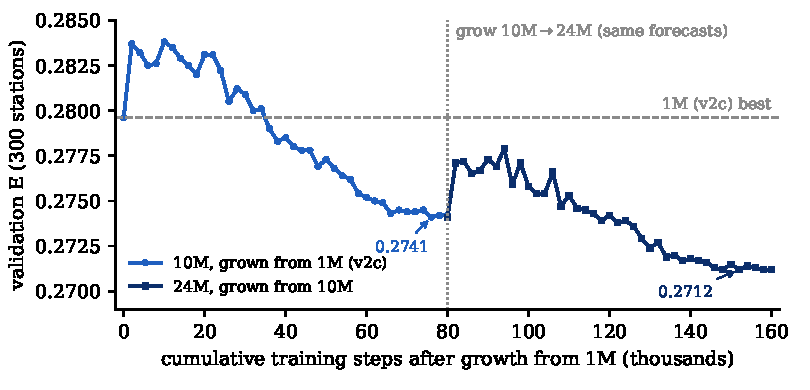
\includegraphics[width=0.82\linewidth]{figures/curve.pdf}
\caption{Validation error on the 300 checking stations through both growths. Each growth starts at its parent's error
(G0). The error rises while the learning rate is high, then falls below the start at step 36,000 (10M) and 38,000 (24M).}
\label{fig:curve}
\end{figure}

\textbf{Growth and adoption.} G0 passed both times (step-0 validation 0.2796 against the parent's 0.2796; 0.2741
against 0.2741). Figure~\ref{fig:curve} shows the curves and Table~\ref{tab:val} the final validation. Both grown models
were adopted, the 24M by a margin of $9\times10^{-5}$ below its bar of 0.27316, which is 0.03\% of $E$. One seed was
run, so this 1\% gain is not robust to seed variation.

\begin{table}[t]
\caption{2022 validation (adoption rule's stations: every 4th station, every 6th hour), MAE per variable and $E$.
$^{\dagger}$The validation pass ran twice (Appendix~\ref{app:dev}); the first pass logged 0.27308, the second 0.27307,
which the result file holds.}
\label{tab:val}
\centering\small
\begin{tabular}{lrrrrrrrr}
\toprule
Model & Params & Temp. & Dew pt. & Wind dir. & Wind spd. & Pressure & $E$ & vs.\ parent\\
\midrule
v2c (1M) & 0.97M & 1.463 & 1.517 & 54.74 & 1.205 & 1.536 & 0.28140 & --\\
10M (grown) & 9.64M & 1.418 & 1.482 & 53.86 & 1.188 & 1.484 & 0.27592 & $-1.95\%$\\
24M (grown) & 24.1M & \textbf{1.388} & \textbf{1.464} & \textbf{53.28} & \textbf{1.177} & \textbf{1.478} & \textbf{0.27307}$^{\dagger}$ & $-1.03\%$\\
\bottomrule
\end{tabular}
\end{table}

\begin{table}[t]
\caption{WEATHER-5K 2023 test, 24 h, MAE (\textdegree C, \textdegree C, degrees, m/s, hPa). Atlas rows: all 5,672
stations, every hourly window ($1.18\times10^9$ scored values per variable), each model scored once. Published rows from
\citet{han2026weather5k}; the comparison with them is by number only.}
\label{tab:test}
\centering\small
\begin{tabular}{lrrrrrr}
\toprule
Model & Params & Temp. & Dew pt. & Wind dir. & Wind spd. & Pressure\\
\midrule
\textbf{Atlas-5K 24M (grown, ours)} & 24.1M & \textbf{1.400} & \textbf{1.468} & \textbf{53.33} & \textbf{1.173} & 1.473\\
Atlas-5K 10M (grown, ours) & 9.64M & 1.429 & 1.486 & 53.93 & 1.183 & 1.477\\
Atlas-5K v2c (ours) & 0.97M & 1.474 & 1.520 & 54.84 & 1.202 & 1.533\\
\midrule
PhysicsFormer, published & 19.3M & 1.55 & 1.59 & 57.37 & 1.21 & 1.43\\
ECMWF-HRES at stations, published & -- & 1.76 & 1.85 & 63.8 & 1.48 & \textbf{0.86}\\
\bottomrule
\end{tabular}
\end{table}

\textbf{2023 test against published models} (Table~\ref{tab:test}). Against PhysicsFormer, the 24M model has lower
error on temperature ($-9.7\%$), dew point ($-7.7\%$), wind direction ($-7.0\%$) and wind speed ($-3.1\%$), and higher
error on pressure ($+3.0\%$). The 10M model shows the same pattern ($-7.8\%$, $-6.6\%$, $-6.0\%$, $-2.2\%$; $+3.3\%$)
with half PhysicsFormer's parameters. Against ECMWF-HRES at the stations, both are 16--21\% lower on four variables
and 71--72\% higher on pressure. The 24M improves on the 10M on every variable of the test year ($-2.1\%$, $-1.2\%$,
$-1.1\%$, $-0.9\%$, $-0.3\%$). Validation and test agree within 1\% for both models.

\subsection{Head-to-head with nine foundation-model configurations}
\label{sec:h2h}

\begin{table}[t]
\caption{Head-to-head windows (709 stations), standardised error $E$ and MAE per variable; lower is better. Opponents
are zero-shot with 512 h of history; Atlas uses 48 h. Both grown Atlas models win all 50 opponent--variable pairs in
both periods (largest Holm-adjusted $p=0.005$). Full paired tables with intervals: Appendix~\ref{app:paired}.}
\label{tab:h2h}
\centering\footnotesize
\setlength{\tabcolsep}{3.6pt}
\begin{tabular}{llrrrrrr}
\toprule
Period & Model & $E$ & Temp. & Dew pt. & Wind dir. & Wind spd. & Pressure\\
\midrule
 2023 test & \textbf{Atlas-5K 24M} (24.1M) & \textbf{0.2742} & \textbf{1.391} & \textbf{1.460} & \textbf{53.93} & \textbf{1.179} & \textbf{1.466}\\
  & Atlas-5K 10M (9.6M) & 0.2770 & 1.420 & 1.475 & 54.51 & 1.190 & 1.472\\
  & Atlas-5K v2c (1M) & 0.2822 & 1.462 & 1.506 & 55.39 & 1.206 & 1.520\\
  & TimesFM 3.0 (Google) & 0.3303 & 1.876 & 1.960 & 63.06 & 1.327 & 1.965\\
  & Chronos-2 multivar. (Amazon) & 0.3313 & 1.843 & 1.920 & 62.79 & 1.335 & 2.067\\
  & TiRex (NX-AI, 35M) & 0.3326 & 1.900 & 1.955 & 64.38 & 1.325 & 1.948\\
  & Chronos-2 (Amazon, 120M) & 0.3343 & 1.899 & 1.965 & 63.39 & 1.349 & 2.027\\
  & TimesFM 2.5 (Google, 200M) & 0.3355 & 1.968 & 1.998 & 63.80 & 1.337 & 2.014\\
  & Sundial (Tsinghua, 128M) & 0.3360 & 1.923 & 2.007 & 64.09 & 1.338 & 2.028\\
  & Chronos-Bolt (Amazon, 205M) & 0.3372 & 1.897 & 2.016 & 64.40 & 1.359 & 1.990\\
  & Time-MoE (200M) & 0.3408 & 1.955 & 2.037 & 65.48 & 1.363 & 1.989\\
  & TTM r2 (IBM, 0.8M) & 0.3647 & 2.175 & 2.155 & 65.79 & 1.359 & 2.827\\
  & Persistence & 0.4361 & 3.738 & 2.224 & 75.69 & 1.724 & 2.785\\
\midrule
 Live 2024--25 & \textbf{Atlas-5K 24M} (24.1M) & \textbf{0.3007} & \textbf{1.421} & \textbf{1.453} & \textbf{64.38} & \textbf{1.202} & 1.624\\
  & Atlas-5K 10M (9.6M) & 0.3028 & 1.448 & 1.469 & 64.76 & 1.210 & \textbf{1.623}\\
  & Atlas-5K v2c (1M) & 0.3071 & 1.487 & 1.498 & 65.40 & 1.227 & 1.655\\
  & TimesFM 3.0 (Google) & 0.3508 & 1.882 & 1.952 & 71.25 & 1.353 & 2.070\\
  & Chronos-2 multivar. (Amazon) & 0.3522 & 1.848 & 1.916 & 70.78 & 1.367 & 2.175\\
  & Chronos-Bolt (Amazon, 205M) & 0.3547 & 1.899 & 2.007 & 71.70 & 1.371 & 2.092\\
  & TiRex (NX-AI, 35M) & 0.3558 & 1.927 & 1.955 & 73.34 & 1.357 & 2.058\\
  & Chronos-2 (Amazon, 120M) & 0.3559 & 1.902 & 1.959 & 71.84 & 1.381 & 2.131\\
  & Sundial (Tsinghua, 128M) & 0.3572 & 1.931 & 1.998 & 72.74 & 1.363 & 2.120\\
  & TimesFM 2.5 (Google, 200M) & 0.3575 & 1.975 & 1.991 & 72.45 & 1.365 & 2.127\\
  & Time-MoE (200M) & 0.3665 & 1.993 & 2.049 & 75.27 & 1.397 & 2.115\\
  & TTM r2 (IBM, 0.8M) & 0.3829 & 2.176 & 2.120 & 74.28 & 1.375 & 2.854\\
  & Persistence & 0.4646 & 3.807 & 2.178 & 87.11 & 1.778 & 2.842\\
\bottomrule
\end{tabular}
\end{table}

\begin{figure}[t]
\centering
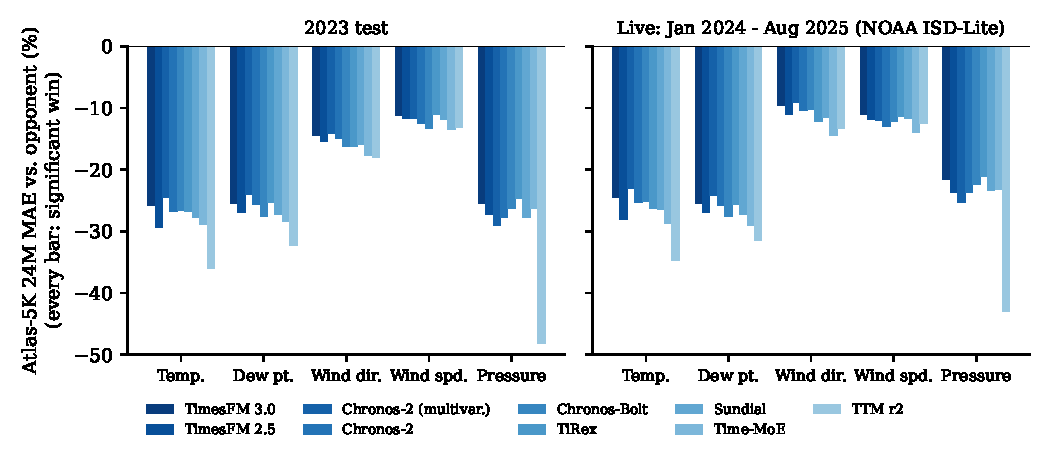
\includegraphics[width=\linewidth]{figures/h2h.pdf}
\caption{Paired difference in MAE, Atlas-5K 24M against each foundation-model configuration, per variable. Every bar is
a significant win after Holm correction over 50 pairs. The 10M model's results are almost the same
(Appendix~\ref{app:paired}).}
\label{fig:h2h}
\end{figure}

Table~\ref{tab:h2h} and Figure~\ref{fig:h2h} give the results. Both grown models win all 50 pairs (ten opponents
$\times$ five variables) on the 2023 test windows and on the live period; the largest Holm-adjusted $p$ is 0.005.
Against the nine foundation-model configurations, the 24M model's per-variable error is 11.0--48.2\% lower on test and
9.1--43.1\% lower on live; for the 10M, 10.2--47.9\% and 8.5--43.1\%. Margins are smallest on wind speed and wind
direction. The closest opponent is TimesFM~3.0: the 24M's $E$ is 17.0\% lower on test and 14.3\% lower on live, and its
per-variable margins on test are $-25.9\%$, $-25.5\%$, $-14.5\%$, $-11.2\%$ and $-25.4\%$, with 95\% intervals that stay
at least 10 points below zero (Appendix~\ref{app:paired}). On the live period every model's error rises (Atlas $E$
+8.8--9.7\%, foundation models +5.0--7.5\%), so the lead narrows, but every win stays significant and the ranking
among opponents barely changes. Even the 1M parent v2c is ahead of every opponent on $E$. Figure~\ref{fig:size} places
the models by size.

\begin{figure}[t]
\centering
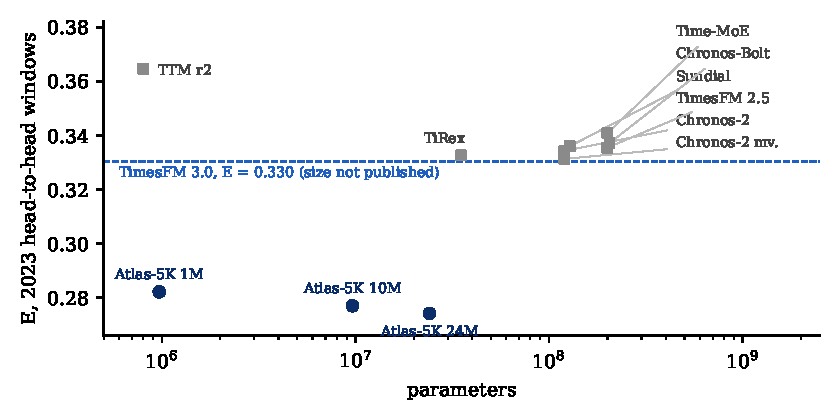
\includegraphics[width=0.78\linewidth]{figures/size.pdf}
\caption{Parameters against $E$ on the 2023 head-to-head windows. TimesFM~3.0's size is not published, so it is drawn
as a line; persistence (no parameters) is omitted.}
\label{fig:size}
\end{figure}

\textbf{24M against 10M.} Paired on the same windows (Holm over five variables), the 24M is significantly better on
all five variables in 2022 validation and on four of five on test and live (Table~\ref{tab:vs10m}). Pressure is a tie on
test ($-0.45\%$, Holm $p=0.017$) and on live ($+0.10\%$, $p=0.56$): the extra parameters improved temperature,
humidity and wind, but not pressure.

\textbf{Harness amendment.} In the first pass three opponents failed for setup reasons. TTM~r2 needs IBM's hourly
frequency token; Sundial and Time-MoE need \texttt{transformers==4.40.1}, which does not install on the runtime's
Python~3.13. We reran them in their documented setup (the token; a Python~3.11 environment), changed nothing else,
and committed the change before the reruns (Appendix~\ref{app:dev}).

\subsection{Pre-registered predictions}
\label{sec:pred}
We made 25 numeric predictions for these runs (Appendix~\ref{app:prereg}, Table~\ref{tab:pred}). Three concern a
size-by-data threshold grid that was planned and not run, so they cannot be scored. Of the other 22, 20 held and 2
failed: for the 10M's validation head-to-head we predicted the smallest margin on pressure, and it was on wind speed;
and we gave the 24M's adoption only 35\%, expecting under 1\% gain from 2.5$\times$ more parameters, but it cleared the
bar by 0.03\% of $E$.

\section{Discussion and limitations}
\label{sec:limits}

\textbf{What the results show.} On WEATHER-5K at 24 hours, a compact model trained for the task and given its
neighbours beats general TSFMs used zero-shot by wide, significant margins, on the test year and on later data; and a
trained model can be grown twice without losing its forecasts, then improved by continued training.

\textbf{What they do not show.}
\begin{itemize}
\item \textbf{Task-trained against zero-shot.} The opponents were not fine-tuned; Atlas is trained on WEATHER-5K's
training years and sees 31 neighbours, while the TSFMs see one station (Chronos-2 multivariate: one station's five
variables). The result is that a small spatial model beats general models \emph{on this problem} as they are offered,
not that it is a better model in general or better than fine-tuned TSFMs.
\item \textbf{Data overlap would favour the opponents, not Atlas.} Several opponents were released in 2025 and their
corpora are not fully documented; they may include NOAA station data from 2023--25. Atlas saw 2014--2021 only.
\item \textbf{Live data differ in processing.} ISD-Lite's hourly selection is not WEATHER-5K's; this is a likely reason
Atlas's error rises more than the opponents' on the live period.
\item \textbf{Size pays little at this scale}, and \textbf{growth against restart is not isolated}: we did not train
10M or 24M models from scratch on WEATHER-5K. \textbf{One seed} per grown model.
\item \textbf{Pressure} is the gap to PhysicsFormer and to ECMWF-HRES; 48 hours of station history hold little of the
large-scale pressure change a global model represents. \textbf{Only 24 h} is reported; no rainfall or extremes.
\item \textbf{Coverage of opponents.} Moirai, Toto, Lag-Llama, MOMENT and other TSFMs were not run. Published models
(PhysicsFormer, ECMWF-HRES) are compared by number, not paired.
\end{itemize}

\textbf{Broader impact.} Better station forecasts from small models can run on modest hardware, which matters for
weather services and users with little compute. The risk is over-trust: a model that beats foundation models on all
five variables is still far worse than operational NWP on pressure and should not replace it. We report that gap
prominently.

\section{Conclusion}
Growing a trained station world model with exact maps, rather than restarting, gave two models that beat nine
foundation-model configurations on every variable, on the test year and on later data, with 5--21$\times$ fewer
parameters than six of the nine. The gains from size were small and absent on pressure; the next step is information the
station history lacks, such as global forecasts as inputs, rather than more parameters.

\section*{Reproducibility statement}
Repository \url{https://github.com/paradoxailab/paradox-world-model} (branch \texttt{main}). Model
\texttt{atlas/atlas/model.py}; growth \texttt{atlas/atlas/grow.py}; training \texttt{atlas/delhi/run\_atlas\_5k.py};
head-to-head \texttt{atlas/delhi/score\_tsfm\_w5k.py}, \texttt{atlas/delhi/pw/opponents.py} and
\texttt{paired\_w5k.py}; live data \texttt{atlas/delhi/tools/fetch\_isd\_live.py}; Colab notebooks in
\texttt{atlas/notebooks/}. Weights: \texttt{models/series/58\_*} (10M) and \texttt{59\_*} (24M), each with its
configuration and results inside. Run logs, result files and paired-test outputs are in
\texttt{atlas/results/colab/atlas5k\_grown/}; every table in this paper is generated from or checked against them by
\texttt{atlas/paper4/make\_tables.py}. NOAA and WEATHER-5K data are downloaded by the scripts and not redistributed.

\bibliographystyle{plainnat}
\bibliography{refs}

\newpage
\appendix
\raggedbottom

\section{Proof of Proposition~\ref{prop:grow}}
\label{app:proofs}

\textbf{Map 1 (width tiling).} Write the parent as a composition of an input map that writes the stream,
$z_0=W_{\text{in}}x$; residual updates $z\mapsto z+g(z)$, where each $g$ reads $\mathrm{LN}(z)$ through linear maps and
writes through a linear map; and decoders that read the stream. We show by induction that every stream state of the
grown model is $[z;z]$ when the parent's is $z$. \emph{Base:} $W'_{\text{in}}=[W_{\text{in}};W_{\text{in}}]$ gives
$[z_0;z_0]$. \emph{LayerNorm:} the mean and variance of $[z;z]$ over $2d$ entries equal those of $z$ over $d$, so with
tiled gain and bias $\mathrm{LN}([z;z])=[\mathrm{LN}(z);\mathrm{LN}(z)]$. \emph{Reading layers:} a weight $W$ that reads
a $d$-vector $u$ becomes $W'=[W/2+\varepsilon,\,W/2-\varepsilon]$, and $W'[u;u]=Wu$. If that layer's output is itself
tiled (the first layer of a block's MLP, whose hidden width doubles), its output rows are tiled too and the argument
repeats for the next layer. \emph{Attention:} each head is duplicated; its query, key and value maps read $[u;u]$ as
above, so both copies compute the parent head's attention weights and values exactly; the geometry-bias network's last
layer is tiled per head; the output projection reads the concatenated heads with halved, $\pm\varepsilon$-perturbed
columns, so its output is the parent's, then tiled. \emph{Writing layers} have tiled rows, so $g'([z;z])=[g(z);g(z)]$
and the residual sum stays tiled. \emph{Decoders} read $[z;z]$ with halved columns, giving the parent's output.
Appended blocks have $B=0$ and add zero. Hence the outputs are identical. With $\varepsilon=0$ the two copies of every
unit would receive identical gradients and stay identical (Net2Net's symmetry); with $\varepsilon\neq0$ their
downstream weights differ, so their gradients do. We use $\varepsilon$ with entries of 5\% of the weights' spread.

\textbf{Map 2 (hidden widening).} For a block $x+B\,\phi(A\,\mathrm{LN}(x))$ with $\phi$ the GELU, set
$A'=[A;A_{\text{new}}]$ and $B'=[B,\,0]$. Then $B'\phi(A'u)=B\phi(Au)+0\cdot\phi(A_{\text{new}}u)=B\phi(Au)$, so the block,
and the network, is unchanged. With upstream gradient $\delta=\partial L/\partial y$ at the block output,
$\partial L/\partial B_{\text{new}}=\delta\,\phi(A_{\text{new}}u)^{\top}$, which is non-zero for generic random
$A_{\text{new}}$, while $\partial L/\partial A_{\text{new}}=\big((B_{\text{new}}^{\top}\delta)\odot\phi'(A_{\text{new}}u)\big)u^{\top}=0$
as long as $B_{\text{new}}=0$. After the first update $B_{\text{new}}\neq0$, and $A_{\text{new}}$ receives gradient. An
appended block with $B=0$ is the identity. $\square$

\section{Data, windows and the error $E$}
\label{app:data}

WEATHER-5K: 5,672 stations, 87,648 hours (2014--2023), five variables (temperature, dew point, wind direction, wind
speed, sea-level pressure), with no missing values after the benchmark's processing. The benchmark's scaler, used for
inputs and for $E$, has means $(12.709, 6.527, 191.189, 3.369, 1014.850)$ and standard deviations
$\sigma=(13.082, 12.139, 99.674, 2.657, 9.175)$. Full test (Table~\ref{tab:test}): every hourly window of 2023 at every
station, 8,689 windows per station, 1,182,816,192 scored values per variable; we score all windows, whereas the
benchmark's loader drops the last incomplete batch. Validation for adoption: every 4th station and every 6th hour of
2022, 49,312,368 values per variable. Training: 2,920 days $\times$ 5,672 stations; an 80,000-step run with 256
neighbourhoods per step sees about 20M of the roughly 400M station-hour windows, so no window repeats.

Head-to-head windows: 2023 test, 709 stations $\times$ 182 starts (2023-01-03 to 2023-12-31); live, 709 stations
$\times$ 145 starts (2024-01-23 to 2025-08-21); up to 3,096,912 (test) and 1,914,220 (live) scored values per variable.

\section{Opponents}
\label{app:opp}

\begin{table}[H]
\centering\scriptsize
\setlength{\tabcolsep}{4pt}
\caption{Opponents as run. All are zero-shot with 512 hourly context values per station and variable, the median (or point) forecast is scored, and no opponent was fine-tuned. Minutes: wall-clock on one A100 for the 2023 test windows. Licences as stated by each model's publisher at the time of the run.}
\label{tab:opp}
\begin{tabular}{lllrrl}
\toprule
Model & Publisher & Params & Context & Minutes & Licence\\
\midrule
TimesFM 3.0 & Google & n/a & 512 & 22.1 & non-commercial research (eval. only)\\
Chronos-2 multivariate & Amazon & 120M & 512 & 7.0 & Apache-2.0\\
TiRex & NX-AI & 35M & 512 & 14.4 & NXAI community (eval. only)\\
Chronos-2 & Amazon & 120M & 512 & 7.5 & Apache-2.0\\
TimesFM 2.5 & Google & 200M & 512 & 5.8 & Apache-2.0\\
Sundial base & Tsinghua THUML & 128M & 512 & 22.5 & Apache-2.0\\
Chronos-Bolt base & Amazon & 205M & 512 & 5.0 & Apache-2.0\\
Time-MoE & Shi et al. & 200M & 512 & 160.2 & Apache-2.0\\
TTM r2 & IBM Research & 0.8M & 512 & 0.2 & Apache-2.0\\
Persistence & -- & 0 & 512 & 0.0 & --\\
\bottomrule
\end{tabular}
\end{table}


Implementation (\texttt{atlas/delhi/pw/opponents.py}, \texttt{score\_tsfm\_w5k.py}): each opponent receives each
station's own 512-hour history per variable (Chronos-2 multivariate: the five variables of a station together),
forward-filled across gaps and back-filled at the start, in physical units, and forecasts 24 hours. The median is
scored: TimesFM~2.5 with its continuous quantile head and quantile-crossing fix; TimesFM~3.0 through its evaluator;
Chronos models through \texttt{predict\_quantiles}; Sundial as the median of 20 sample paths; Time-MoE as its point
forecast; TTM~r2 with the 512-hour model chosen by IBM's selector and hourly frequency token 7; TiRex's 0.5 quantile.
No opponent output is used for training, and nothing is tuned on test or live data.

\section{Live data and the identity check}
\label{app:live}

\texttt{fetch\_isd\_live.py} downloads ISD-Lite (hourly, the observation nearest each hour) for the 5,672 stations from
NOAA's open-data bucket (\texttt{noaa-isd-pds}); NCEI's older path served a web page, and the switch was committed before
any live score. The bucket's newest files are dated 30 August 2025, so the live period ends on 24 August 2025, the last
day that half the reporting stations cover. Truth is observed hours only; model inputs are the same series with the last
observation carried forward (no later value fills an earlier hour), for every model alike. For the 24M round the data
were rebuilt with a fixed end hour (\texttt{--end 2025-08-24T23}). The pre-registered check re-scored the 10M model on
the rebuilt data and compared per-window counts and errors with those saved in the first live round: they were
identical (\texttt{LIVE DATA IDENTICAL TO PHASE 5b: True}), so the earlier opponents' saved errors could be reused.

\section{Statistical tests}
\label{app:stats}

For a pair (our model $a$, opponent $b$) and variable $v$, let $A_s$ and $B_s$ be the summed absolute errors and $c_s$
the count over window cells of station $s$ that \emph{both} models scored. Then $\mathrm{MAE}_a=\sum_s A_s/\sum_s c_s$.
The bootstrap draws the 709 stations with replacement 10,000 times and computes
$\Delta^{*}=\sum (A^{*}-B^{*})/\sum c^{*}$; the two-sided $p$ is
$\min\!\big(1,\,2\min(\Pr[\Delta^{*}\ge0],\Pr[\Delta^{*}\le0])+10^{-4}\big)$, and the 95\% interval is the 2.5--97.5\%
quantiles of $\Delta^{*}/\mathrm{MAE}_b$. The Diebold--Mariano test uses the daily mean loss difference over stations
with Newey--West variance at lag $\mathrm{round}(T^{1/3})$. Because the paired MAEs use only cells both models scored,
they can differ from Table~\ref{tab:h2h}'s by at most 0.004\% relative. The $p$ used is $\max(p_{\text{boot}},p_{\text{DM}})$,
Holm-corrected over each family of 50 pairs (one of our models, one period), $\alpha=0.01$; the 24M-against-10M
comparison is a family of five.

\emph{Resolution of the bootstrap.} With 10,000 resamples the smallest bootstrap $p$ is $10^{-4}$, so Holm over 50 gives
at best 0.005, which every pair reached; the Diebold--Mariano $p$-values are far smaller. Had all four families been
pooled into one of 200 pairs, the bootstrap's resolution alone would cap the adjusted $p$ at 0.02, above $\alpha$. The
family definition was fixed before the runs; a claim over a pooled family would need more resamples.

\section{Full paired results}
\label{app:paired}

\begin{table}[h]
\centering\scriptsize
\setlength{\tabcolsep}{3pt}
\caption{Atlas-5K 24M against each opponent, 2023 test: paired MAE difference in \% with the 95\% station-block bootstrap interval. All 50 of 50 pairs are significant wins (largest Holm-adjusted $p=0.005$).}
\label{tab:paired_atlas25m_test}
\begin{tabular}{lccccc}
\toprule
Opponent & Temp. & Dew pt. & Wind dir. & Wind spd. & Pressure\\
\midrule
TimesFM 3.0 & $-25.9$ [-27.2, -24.6] & $-25.5$ [-26.8, -24.3] & $-14.5$ [-15.3, -13.7] & $-11.2$ [-11.9, -10.5] & $-25.4$ [-26.6, -24.3]\\
Chronos-2 multivariate & $-24.6$ [-25.8, -23.3] & $-24.0$ [-25.2, -22.8] & $-14.1$ [-14.9, -13.3] & $-11.7$ [-12.4, -10.9] & $-29.1$ [-30.3, -27.9]\\
TiRex & $-26.8$ [-28.1, -25.5] & $-25.4$ [-26.6, -24.1] & $-16.2$ [-17.0, -15.4] & $-11.0$ [-11.7, -10.3] & $-24.8$ [-25.9, -23.6]\\
Chronos-2 & $-26.8$ [-28.1, -25.5] & $-25.7$ [-27.0, -24.5] & $-14.9$ [-15.8, -14.1] & $-12.6$ [-13.4, -11.8] & $-27.7$ [-28.9, -26.5]\\
TimesFM 2.5 & $-29.3$ [-30.7, -28.0] & $-26.9$ [-28.2, -25.7] & $-15.5$ [-16.2, -14.7] & $-11.8$ [-12.5, -11.1] & $-27.2$ [-28.4, -26.1]\\
Sundial base & $-27.7$ [-29.1, -26.4] & $-27.3$ [-28.6, -26.0] & $-15.9$ [-16.6, -15.1] & $-11.9$ [-12.6, -11.2] & $-27.7$ [-28.9, -26.6]\\
Chronos-Bolt base & $-26.7$ [-28.0, -25.4] & $-27.6$ [-28.9, -26.3] & $-16.3$ [-17.1, -15.5] & $-13.3$ [-14.1, -12.5] & $-26.4$ [-27.6, -25.2]\\
Time-MoE & $-28.9$ [-30.2, -27.6] & $-28.4$ [-29.6, -27.1] & $-17.6$ [-18.4, -16.9] & $-13.5$ [-14.2, -12.8] & $-26.3$ [-27.5, -25.2]\\
TTM r2 & $-36.1$ [-37.6, -34.6] & $-32.3$ [-33.6, -31.0] & $-18.0$ [-18.8, -17.3] & $-13.2$ [-13.9, -12.6] & $-48.2$ [-49.8, -46.5]\\
Persistence & $-62.8$ [-65.3, -60.4] & $-34.4$ [-35.6, -33.1] & $-28.8$ [-29.6, -27.9] & $-31.6$ [-32.9, -30.4] & $-47.4$ [-48.8, -45.9]\\
\bottomrule
\end{tabular}
\end{table}

\begin{table}[h]
\centering\scriptsize
\setlength{\tabcolsep}{3pt}
\caption{Atlas-5K 24M against each opponent, Live, Jan 2024 -- Aug 2025: paired MAE difference in \% with the 95\% station-block bootstrap interval. All 50 of 50 pairs are significant wins (largest Holm-adjusted $p=0.005$).}
\label{tab:paired_atlas25m_live}
\begin{tabular}{lccccc}
\toprule
Opponent & Temp. & Dew pt. & Wind dir. & Wind spd. & Pressure\\
\midrule
TimesFM 3.0 & $-24.5$ [-25.8, -23.2] & $-25.6$ [-26.8, -24.2] & $-9.6$ [-10.7, -8.6] & $-11.1$ [-11.9, -10.3] & $-21.6$ [-22.7, -20.4]\\
Chronos-2 multivariate & $-23.1$ [-24.2, -22.0] & $-24.1$ [-25.3, -22.9] & $-9.1$ [-10.2, -7.9] & $-12.1$ [-12.8, -11.3] & $-25.3$ [-26.5, -24.1]\\
TiRex & $-26.2$ [-27.5, -25.0] & $-25.6$ [-26.9, -24.3] & $-12.2$ [-13.3, -11.1] & $-11.4$ [-12.2, -10.7] & $-21.1$ [-22.2, -19.9]\\
Chronos-2 & $-25.3$ [-26.6, -24.0] & $-25.8$ [-27.1, -24.5] & $-10.4$ [-11.5, -9.3] & $-13.0$ [-13.8, -12.1] & $-23.8$ [-25.0, -22.6]\\
TimesFM 2.5 & $-28.1$ [-29.4, -26.7] & $-27.0$ [-28.3, -25.7] & $-11.2$ [-12.2, -10.1] & $-11.9$ [-12.7, -11.2] & $-23.7$ [-24.8, -22.5]\\
Sundial base & $-26.4$ [-27.7, -25.1] & $-27.2$ [-28.6, -25.9] & $-11.5$ [-12.4, -10.6] & $-11.8$ [-12.5, -11.0] & $-23.4$ [-24.5, -22.2]\\
Chronos-Bolt base & $-25.1$ [-26.4, -23.8] & $-27.6$ [-28.9, -26.2] & $-10.2$ [-11.2, -9.2] & $-12.3$ [-13.1, -11.5] & $-22.4$ [-23.5, -21.2]\\
Time-MoE & $-28.7$ [-30.0, -27.3] & $-29.1$ [-30.4, -27.7] & $-14.5$ [-15.3, -13.6] & $-13.9$ [-14.6, -13.2] & $-23.2$ [-24.3, -22.1]\\
TTM r2 & $-34.7$ [-36.2, -33.2] & $-31.5$ [-32.9, -30.0] & $-13.3$ [-14.2, -12.4] & $-12.5$ [-13.3, -11.8] & $-43.1$ [-44.6, -41.6]\\
Persistence & $-62.7$ [-65.5, -60.0] & $-33.3$ [-34.6, -31.9] & $-26.1$ [-27.1, -25.1] & $-32.4$ [-33.8, -31.0] & $-42.8$ [-44.1, -41.5]\\
\bottomrule
\end{tabular}
\end{table}

\begin{table}[h]
\centering\scriptsize
\setlength{\tabcolsep}{3pt}
\caption{Atlas-5K 10M against each opponent, 2023 test: paired MAE difference in \% with the 95\% station-block bootstrap interval. All 50 of 50 pairs are significant wins (largest Holm-adjusted $p=0.005$).}
\label{tab:paired_atlas10m_test}
\begin{tabular}{lccccc}
\toprule
Opponent & Temp. & Dew pt. & Wind dir. & Wind spd. & Pressure\\
\midrule
TimesFM 3.0 & $-24.3$ [-25.6, -23.1] & $-24.8$ [-26.0, -23.5] & $-13.6$ [-14.4, -12.7] & $-10.4$ [-11.1, -9.7] & $-25.1$ [-26.3, -23.9]\\
Chronos-2 multivariate & $-23.0$ [-24.2, -21.8] & $-23.2$ [-24.3, -22.0] & $-13.2$ [-14.0, -12.4] & $-10.9$ [-11.6, -10.2] & $-28.8$ [-30.0, -27.6]\\
TiRex & $-25.3$ [-26.5, -24.0] & $-24.6$ [-25.8, -23.3] & $-15.3$ [-16.1, -14.5] & $-10.2$ [-10.9, -9.5] & $-24.4$ [-25.6, -23.3]\\
Chronos-2 & $-25.2$ [-26.5, -23.9] & $-25.0$ [-26.2, -23.7] & $-14.0$ [-14.8, -13.2] & $-11.8$ [-12.6, -11.0] & $-27.4$ [-28.6, -26.2]\\
TimesFM 2.5 & $-27.8$ [-29.2, -26.5] & $-26.2$ [-27.4, -24.9] & $-14.6$ [-15.3, -13.8] & $-11.0$ [-11.7, -10.3] & $-26.9$ [-28.1, -25.7]\\
Sundial base & $-26.2$ [-27.5, -24.9] & $-26.5$ [-27.8, -25.3] & $-14.9$ [-15.7, -14.2] & $-11.1$ [-11.8, -10.4] & $-27.4$ [-28.6, -26.2]\\
Chronos-Bolt base & $-25.2$ [-26.5, -23.9] & $-26.8$ [-28.1, -25.6] & $-15.4$ [-16.2, -14.6] & $-12.5$ [-13.3, -11.7] & $-26.0$ [-27.2, -24.9]\\
Time-MoE & $-27.4$ [-28.7, -26.1] & $-27.6$ [-28.8, -26.4] & $-16.8$ [-17.5, -16.0] & $-12.7$ [-13.4, -12.1] & $-26.0$ [-27.2, -24.9]\\
TTM r2 & $-34.7$ [-36.2, -33.3] & $-31.6$ [-32.9, -30.3] & $-17.1$ [-17.9, -16.4] & $-12.4$ [-13.1, -11.8] & $-47.9$ [-49.6, -46.3]\\
Persistence & $-62.0$ [-64.5, -59.6] & $-33.7$ [-34.9, -32.4] & $-28.0$ [-28.8, -27.2] & $-31.0$ [-32.2, -29.8] & $-47.1$ [-48.6, -45.7]\\
\bottomrule
\end{tabular}
\end{table}

\begin{table}[H]
\centering\scriptsize
\setlength{\tabcolsep}{2.4pt}
\caption{Atlas-5K 10M against each opponent, Live, Jan 2024 -- Aug 2025: paired MAE difference in \% with the 95\% station-block bootstrap interval. All 50 of 50 pairs are significant wins (largest Holm-adjusted $p=0.005$).}
\label{tab:paired_atlas10m_live}
\begin{tabular}{lccccc}
\toprule
Opponent & Temp. & Dew pt. & Wind dir. & Wind spd. & Pressure\\
\midrule
TimesFM 3.0 & $-23.1$ [-24.4, -21.8] & $-24.7$ [-26.0, -23.4] & $-9.1$ [-10.2, -8.0] & $-10.5$ [-11.3, -9.8] & $-21.6$ [-22.8, -20.5]\\
Chronos-2 multivariate & $-21.7$ [-22.8, -20.5] & $-23.3$ [-24.5, -22.1] & $-8.5$ [-9.6, -7.4] & $-11.5$ [-12.2, -10.7] & $-25.4$ [-26.6, -24.2]\\
TiRex & $-24.8$ [-26.1, -23.6] & $-24.8$ [-26.1, -23.5] & $-11.7$ [-12.7, -10.6] & $-10.8$ [-11.5, -10.1] & $-21.1$ [-22.3, -20.0]\\
Chronos-2 & $-23.9$ [-25.1, -22.6] & $-25.0$ [-26.3, -23.7] & $-9.9$ [-10.9, -8.8] & $-12.4$ [-13.2, -11.6] & $-23.9$ [-25.1, -22.7]\\
TimesFM 2.5 & $-26.7$ [-28.0, -25.4] & $-26.2$ [-27.5, -24.9] & $-10.6$ [-11.6, -9.6] & $-11.3$ [-12.1, -10.6] & $-23.7$ [-24.9, -22.6]\\
Sundial base & $-25.0$ [-26.3, -23.7] & $-26.5$ [-27.8, -25.1] & $-11.0$ [-11.9, -10.1] & $-11.2$ [-11.9, -10.4] & $-23.4$ [-24.6, -22.3]\\
Chronos-Bolt base & $-23.7$ [-25.0, -22.4] & $-26.8$ [-28.1, -25.4] & $-9.7$ [-10.7, -8.7] & $-11.7$ [-12.5, -10.9] & $-22.4$ [-23.6, -21.3]\\
Time-MoE & $-27.3$ [-28.6, -26.0] & $-28.3$ [-29.6, -26.9] & $-14.0$ [-14.7, -13.2] & $-13.4$ [-14.0, -12.7] & $-23.3$ [-24.4, -22.2]\\
TTM r2 & $-33.5$ [-35.0, -31.9] & $-30.7$ [-32.1, -29.2] & $-12.8$ [-13.7, -11.9] & $-12.0$ [-12.7, -11.2] & $-43.1$ [-44.7, -41.6]\\
Persistence & $-62.0$ [-64.7, -59.3] & $-32.5$ [-33.8, -31.2] & $-25.7$ [-26.6, -24.7] & $-31.9$ [-33.3, -30.6] & $-42.9$ [-44.2, -41.6]\\
\bottomrule
\end{tabular}
\end{table}

\begin{table}[H]
\centering\scriptsize
\setlength{\tabcolsep}{3pt}
\caption{Atlas-5K 24M against its parent 10M, paired on identical windows: MAE difference in \%, 95\% bootstrap interval, and Holm-adjusted $p$ (over the five variables). Validation: the adoption rule's 2022 stations.}
\label{tab:vs10m}
\begin{tabular}{lccccc}
\toprule
Period & Temp. & Dew pt. & Wind dir. & Wind spd. & Pressure\\
\midrule
2022 validation & $-2.12$ [-2.26, -1.98] & $-1.19$ [-1.29, -1.09] & $-1.10$ [-1.19, -1.02] & $-0.93$ [-1.01, -0.84] & $-0.42$ [-0.57, -0.28]\\
 & $p=0.0005$ & $p=0.0005$ & $p=0.0005$ & $p=0.0005$ & $p=0.0016$\\[2pt]
2023 test & $-2.06$ [-2.20, -1.93] & $-1.04$ [-1.16, -0.92] & $-1.07$ [-1.15, -0.98] & $-0.90$ [-0.99, -0.82] & $-0.45$ [-0.60, -0.31]\\
 & $p=0.0005$ & $p=0.0005$ & $p=0.0005$ & $p=0.0005$ & $p=0.017$ (tie)\\[2pt]
Live 2024--25 & $-1.86$ [-2.01, -1.70] & $-1.08$ [-1.20, -0.95] & $-0.59$ [-0.70, -0.48] & $-0.66$ [-0.75, -0.58] & $+0.10$ [-0.08, +0.28]\\
 & $p=0.0005$ & $p=0.0005$ & $p=0.0005$ & $p=0.0005$ & $p=0.56$ (tie)\\[2pt]
\bottomrule
\end{tabular}
\end{table}


\section{Training details and compute}
\label{app:train}

\begin{table}[H]
\caption{Architecture, training and compute of the three Atlas-5K models.}
\label{tab:train}
\centering\small
\begin{tabular}{lrrr}
\toprule
 & v2c (1M) & 10M & 24M\\
\midrule
Width $d$ / heads & 196 / 4 & 392 / 8 & 392 / 8\\
Encoder + dynamics blocks & 2 + 2 & 7 + 7 & 8 + 7\\
Block hidden width & 392 & 784 & 1,960\\
Parameters & 968,672 & 9,639,780 & 24,103,796\\
Initialisation & random & v2c, Map 1 & 10M, Map 2\\
Peak learning rate & $10^{-3}$ & $3\times10^{-4}$ & $2\times10^{-4}$\\
Steps after growth (batch 256 neighbourhoods) & -- & 80,000 & 80,000\\
Best checkpoint: step (300-station val.) & -- & 76,000 (0.2741) & 72,000 (0.2712)\\
Hardware & -- & A100 80GB & A100, then L4\\
Training time & -- & 103.4 min & 12.4 + 355.8 min\\
\bottomrule
\end{tabular}
\end{table}

Shared settings: pinball loss on quantiles 0.1/0.5/0.9 plus $0.2\times$ masked-input reconstruction (15\% of
observed inputs hidden); AdamW, weight decay $10^{-4}$; one-cycle schedule with 3\% warm-up; gradient clipping 1.0;
float16 mixed precision; validation every 2,000 steps on 300 fixed stations (every 6th hour of 2022); patience 8
checks; seed 600. The 24M ran steps 0--8,000 on an A100 (0.075\,s/step) and resumed from its full checkpoint (model,
optimiser, schedule, step) on an L4 for steps 8,000--80,000 (0.220\,s/step). Compute for this paper's runs, all on Google
Colab: about 2.5 A100-hours for the 10M (training, validation and two test scorings); about 6 L4-hours and 0.2
A100-hours for the 24M's training; about 7.5 A100-hours for the 24M's evaluation and the widened head-to-head (Time-MoE
alone 4.8 hours over both periods). The opponent runs of the 10M round are logged in the repository and not summed here.

\section{Pre-registration timeline and every prediction}
\label{app:prereg}

\begin{table}[H]
\caption{Commits to the public repository (UTC). Each fixes rules or predictions before the result it governs existed.}
\label{tab:timeline}
\centering\scriptsize
\begin{tabular}{lll}
\toprule
When & Commit & Content\\
\midrule
2026-11-16 23:52 & \texttt{84e14b9} & 10M rules (G0, adoption bar 0.2786, test only if adopted) and 8 predictions\\
2026-11-17 02:56 & \texttt{e09e239} & 10M adopted; 2023 test scored once\\
2026-11-17 09:03 & \texttt{9d5f778} & Head-to-head rules, opponents, tests, threshold-grid plan and 6 predictions\\
2026-11-17 09:27 & \texttt{3e03ed2} & Amendment before any opponent score: every 8th station, every 2nd day (cost)\\
2026-11-17 12:33 & \texttt{f9be24d} & 2023 test and live-data rules, 4 predictions\\
2026-11-17 14:44 & \texttt{79227ce} & Live-data source amendment, before any live score\\
2026-11-17 17:33 & \texttt{2b1950e} & 24M rules (bar 0.27316, test regardless), four new opponents, data check, 7 predictions\\
2026-11-18 09:57 & \texttt{396433f} & 24M training and adoption (validation only)\\
2026-11-18 11:48 & \texttt{ab4726c} & Harness fixes for TTM, Sundial, Time-MoE, before their reruns\\
2026-11-18 17:39 & \texttt{a8d51fb} & 24M 2023 test and widened head-to-head; predictions scored\\
\bottomrule
\end{tabular}
\end{table}

\begin{table}[H]
\caption{Every numeric prediction for these runs, with the probability written before the run and the outcome.}
\label{tab:pred}
\centering\scriptsize
\begin{tabular}{p{0.64\linewidth}rl}
\toprule
Prediction & Prob. & Outcome\\
\midrule
\multicolumn{3}{l}{\emph{10M (commit 84e14b9)}}\\
G0 passes & 95\% & held\\
10M adopted & 60\% & held\\
If adopted, validation $E$ in $[0.270,0.278]$ & 60\% & held (0.2759)\\
v2c beats PhysicsFormer on 2023 (four of five variables) & 60\% & held\\
v2c's pressure MAE stays above PhysicsFormer's & 90\% & held\\
10M beats PhysicsFormer on 2023 & 75\% & held\\
10M's pressure MAE above 1.43 & 75\% & held (1.477)\\
Neither beats ECMWF-HRES (four-variable rule) & 95\% & held\\
\multicolumn{3}{l}{\emph{Head-to-head on 2022 validation and threshold grid (commit 9d5f778)}}\\
10M lower than TimesFM 2.5, TimesFM 3.0 and Chronos-2 on all five variables & 85\% & held\\
Largest margin on wind direction or dew point, smallest on pressure & 60\% & \textbf{failed} (smallest: wind speed)\\
Chronos-2 multivariate better than univariate on $E$ & 55\% & held (0.3327 vs 0.3359)\\
Threshold form B verified & 55\% & not scored (grid not run)\\
At all data, 10M from scratch beats 1M from scratch & 60\% & not scored (grid not run)\\
Minimum size that beats TimesFM 2.5 at all data $\le$1M & 70\% & not scored (grid not run)\\
\multicolumn{3}{l}{\emph{2023 test and live (commit f9be24d)}}\\
10M wins all 30 pairs on 2023 & 90\% & held\\
10M wins all 30 pairs on live & 80\% & held\\
Atlas's live $E$ at least 3\% above its 2023 $E$ & 55\% & held (+9.3\%)\\
v2c wins all 30 pairs on both periods & 75\% & held\\
\multicolumn{3}{l}{\emph{24M (commit 2b1950e)}}\\
G0 passes & 90\% & held\\
24M adopted & 35\% & \textbf{failed} (adopted)\\
Validation $E$ in $[0.268,0.276]$ & 70\% & held (0.27307)\\
24M wins 50 of 50 on both periods & 80\% & held\\
No new opponent's test $E$ below 0.31 & 80\% & held (best 0.3326)\\
Best new opponent is TiRex or Sundial & 60\% & held (TiRex)\\
24M significantly better than 10M on $\ge$3 of 5 variables (test) & 50\% & held (4)\\
\bottomrule
\end{tabular}
\end{table}

\section{Deviations and incidents}
\label{app:dev}

\begin{itemize}
\item \textbf{Harness amendment} (commit \texttt{ab4726c}, before the reruns). TTM~r2 raised ``Expecting freq\_token''
and was given IBM's hourly token; Sundial and Time-MoE failed inside their remote code on a newer \texttt{transformers}
(\texttt{DynamicCache.seen\_tokens}) and were run in a Python~3.11 environment with their documented
\texttt{transformers==4.40.1}. Windows, history and scoring were unchanged. The 24M rules said an opponent that fails in
its documented setup is reported as not scored; these three ran in their documented setup.
\item \textbf{Head-to-head subsampling} (commit \texttt{3e03ed2}, before any opponent score): every 8th station and every
2nd day, for cost. An interrupted run on the full window set had scored only Atlas and persistence; those numbers are
recorded in the repository and not used.
\item \textbf{Threshold grid not run.} The size-by-data grid planned in commit \texttt{9d5f778} was not run; its
predictions are left unscored and no threshold-function claim is made.
\item \textbf{Training interruptions (24M).} We once deleted the Colab runtime while it was training (its display was
stuck); the run resumed from its step-8,000 checkpoint with no loss of progress, and a duplicate session was stopped
after checking file times. The resume moved the run from an A100 to an L4. A later session died during the 2023 test
(the host computer slept); the evaluation was rerun on an A100 from the finished checkpoint.
\item \textbf{Validation rerun.} Because of that rerun, the 24M's final validation ran twice: $E=0.27308$ and then
$0.27307$ (wind direction 53.2820 against 53.2819, from GPU summation order). The verdict is the same; the result file
holds 0.27307, and the repository's first report of 0.27308 carries a dated correction.
\end{itemize}

\section{Assets and licences}
\label{app:assets}
WEATHER-5K \citep{han2026weather5k} (built from NOAA ISD \citep{smith2011isd}); NOAA ISD-Lite from NOAA's open-data
bucket (public). TimesFM~2.5, Chronos-Bolt, Chronos-2, Sundial, Time-MoE and TTM~r2 under Apache-2.0; TimesFM~3.0 under
a non-commercial research licence and TiRex under the NXAI community licence, both used for evaluation only and not
redistributed. Our code and weights: Apache-2.0. No personal data are involved.

\newpage
\section*{NeurIPS Paper Checklist}

\begin{enumerate}[leftmargin=1.5em,itemsep=3pt]
\item \textbf{Claims.} Do the main claims in the abstract and introduction accurately reflect the paper's contributions
and scope? \answerYes{} The abstract states the setting (WEATHER-5K, 24 h, zero-shot opponents), the pressure gap and
the small gain from size; Section~\ref{sec:limits} states what is not shown.
\item \textbf{Limitations.} \answerYes{} Section~\ref{sec:limits}: zero-shot opponents, possible data overlap, live-data
processing, one seed, growth against restart not isolated, pressure, 24 h only, opponents not run.
\item \textbf{Theory assumptions and proofs.} \answerYes{} Proposition~\ref{prop:grow} states its assumptions (exact
arithmetic, the stated parameter maps); Appendix~\ref{app:proofs} gives the proof, and the measured floating-point
difference is reported.
\item \textbf{Experimental result reproducibility.} \answerYes{} Protocol in Section~\ref{sec:protocol}, details in
Appendices~\ref{app:data}--\ref{app:train}, code and notebooks in the repository.
\item \textbf{Open access to data and code.} \answerYes{} Code, rules, logs, per-window paired results and weights are
public; WEATHER-5K and NOAA data are public and downloaded by the scripts.
\item \textbf{Experimental setting/details.} \answerYes{} Appendix~\ref{app:train} (optimiser, schedule, steps, batch,
selection by validation only) and Appendix~\ref{app:opp} (opponent settings).
\item \textbf{Experiment statistical significance.} \answerYes{} Station-block bootstrap intervals and
Diebold--Mariano tests with Holm correction (Appendices~\ref{app:stats}, \ref{app:paired}); the single-seed limitation is
stated.
\item \textbf{Experiments compute resources.} \answerYes{} Appendix~\ref{app:train}.
\item \textbf{Code of ethics.} \answerYes{} Public weather data and public models used under their licences.
\item \textbf{Broader impacts.} \answerYes{} Section~\ref{sec:limits}, ``Broader impact''.
\item \textbf{Safeguards.} \answerNA{} The released models forecast station weather and pose no high risk of misuse.
\item \textbf{Licences for existing assets.} \answerYes{} Appendix~\ref{app:assets} and Table~\ref{tab:opp}.
\item \textbf{New assets.} \answerYes{} Weights and code are documented in the repository's model card
(\texttt{atlas/MODELS.md}), with checksums.
\item \textbf{Crowdsourcing and research with human subjects.} \answerNA{}
\item \textbf{IRB approvals.} \answerNA{}
\item \textbf{Declaration of LLM usage.} \answerYes{} An LLM-based assistant (Claude) was used to write and run code,
operate the cloud notebooks and draft text. All numbers come from logged runs and are checked against the result files
by script (\texttt{make\_tables.py --check}). The method itself does not involve LLMs.
\end{enumerate}

\end{document}
